\subsection{Scenario 1: No Changes}
\textit{In this scenario, no external changes are made to the infrastructure. The purpose of this scenario is to see how the system behaves when no changes are made.}

To introduce the graphs and explain their significance, this subsection will delve into the graphs in more detail than in the subsequent subsections. 

\begin{figure}[H]
    \centering
    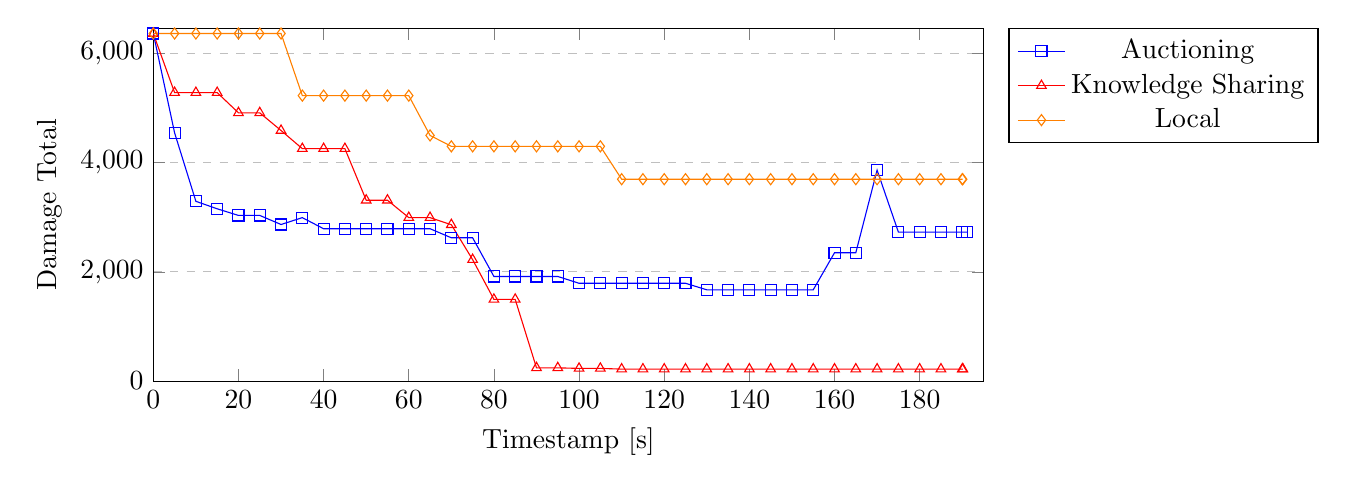
\begin{tikzpicture}
\begin{axis}[
    xlabel={Timestamp [s]},
    ylabel={Damage Total},
    xmin=0, xmax=195000,
    ymin=0, ymax=6464,
    legend pos=outer north east,
    ymajorgrids=true,
    grid style=dashed,
    width=\textwidth,
    height=0.5\textwidth,
    scaled x ticks=base 10:-3,
    xtick scale label code/.code={}
]

	\addplot[color=blue,mark=square] coordinates {
        (0,6367.26)(5000,4547.28)(10000,3293.02)(15000,3156.13)(20000,3034.57)(25000,3034.57)(30000,2868.58)(35000,2993.93)(40000,2790.80)(45000,2790.80)(50000,2790.80)(55000,2790.80)(60000,2790.80)(65000,2790.80)(70000,2624.98)(75000,2624.98)(80000,1916.52)(85000,1916.52)(90000,1916.52)(95000,1916.52)(100000,1791.72)(105000,1791.72)(110000,1791.72)(115000,1791.72)(120000,1791.72)(125000,1791.72)(130000,1671.71)(135000,1671.71)(140000,1671.71)(145000,1671.71)(150000,1671.71)(155000,1671.71)(160000,2351.16)(165000,2351.16)(170000,3864.46)(175000,2729.60)(180000,2729.60)(185000,2729.60)(190000,2729.60)(191066,2729.60)
    };
    \addlegendentry{Auctioning}
	\addplot[color=red,mark=triangle] coordinates {
        (0,6367.26)(5000,5284.52)(10000,5284.52)(15000,5284.52)(20000,4914.13)(25000,4914.13)(30000,4590.69)(35000,4257.62)(40000,4257.62)(45000,4257.62)(50000,3313.54)(55000,3313.54)(60000,2994.50)(65000,2994.50)(70000,2864.46)(75000,2224.62)(80000,1496.52)(85000,1496.52)(90000,242.72)(95000,242.72)(100000,232.18)(105000,232.18)(110000,219.25)(115000,219.25)(120000,219.25)(125000,219.25)(130000,219.25)(135000,219.25)(140000,219.25)(145000,219.25)(150000,219.25)(155000,219.25)(160000,219.25)(165000,219.25)(170000,219.25)(175000,219.25)(180000,219.25)(185000,219.25)(190000,219.25)(190155,219.25)
    };
    \addlegendentry{Knowledge Sharing}
	\addplot[color=orange,mark=diamond] coordinates {
        (0,6367.26)(5000,6367.26)(10000,6367.26)(15000,6367.26)(20000,6367.26)(25000,6367.26)(30000,6367.26)(35000,5229.23)(40000,5229.23)(45000,5229.23)(50000,5229.23)(55000,5229.23)(60000,5229.23)(65000,4499.97)(70000,4300.22)(75000,4300.22)(80000,4300.22)(85000,4300.22)(90000,4300.22)(95000,4300.22)(100000,4300.22)(105000,4300.22)(110000,3698.17)(115000,3698.17)(120000,3698.17)(125000,3698.17)(130000,3698.17)(135000,3698.17)(140000,3698.17)(145000,3698.17)(150000,3698.17)(155000,3698.17)(160000,3698.17)(165000,3698.17)(170000,3698.17)(175000,3698.17)(180000,3698.17)(185000,3698.17)(190000,3698.17)(190110,3698.17)
    };
    \addlegendentry{Local}




\end{axis}
\end{tikzpicture}
    \caption{This graph shows the overall damage of the system in the scenario where no changes are made overtime.}
    \label{fig:overall-damage-no-change}
\end{figure}

From Figure \ref{fig:overall-damage-no-change} we see that the agent with the Local-feature set (from here-on \textit{local-agent}) slowly reduces the overall damage of the network, but is unable to get any lower than around $275$, and stays at this value after roughly the first $50$ seconds.
Within the first $25$ seconds, the knowledge-sharing agents are able to reduce the overall damage to around $220$, but is unable to get any lower than this. 
Finally, the auctioning are able to reduce the damage to roughly $80$, but is only able to get there after $80$ seconds.
The lowest value is for the auctioning agent at $35\%$ of the damage the local-agent.

\begin{figure}[H]
    \centering
    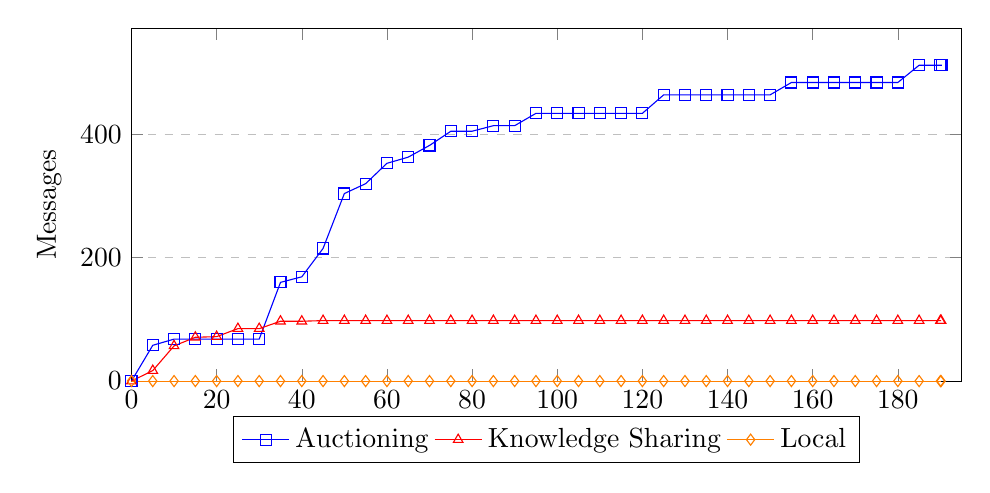
\begin{tikzpicture}
\begin{axis}[
    xlabel={Timestamp [s]},
    ylabel={Messages},
    xmin=0, xmax=195000,
    ymin=0, ymax=572,
    legend columns=-1,
    legend style={at={(0.5,-0.1)},anchor=north},
    ymajorgrids=true,
    grid style=dashed,
    width=\textwidth,
    height=0.5\textwidth,
    scaled x ticks=base 10:-3,
    xtick scale label code/.code={}
]

	\addplot[color=blue,mark=square] coordinates {
        (0,0)(5000,58)(10000,68)(15000,68)(20000,68)(25000,68)(30000,68)(35000,160)(40000,169)(45000,215)(50000,304)(55000,320)(60000,353)(65000,363)(70000,382)(75000,405)(80000,405)(85000,414)(90000,414)(95000,434)(100000,434)(105000,434)(110000,434)(115000,434)(120000,434)(125000,464)(130000,464)(135000,464)(140000,464)(145000,464)(150000,464)(155000,484)(160000,484)(165000,484)(170000,484)(175000,484)(180000,484)(185000,512)(190000,512)(190364,512)
    };
    \addlegendentry{Auctioning}
	\addplot[color=red,mark=triangle] coordinates {
        (0,0)(5000,17)(10000,57)(15000,71)(20000,72)(25000,85)(30000,85)(35000,97)(40000,97)(45000,98)(50000,98)(55000,98)(60000,98)(65000,98)(70000,98)(75000,98)(80000,98)(85000,98)(90000,98)(95000,98)(100000,98)(105000,98)(110000,98)(115000,98)(120000,98)(125000,98)(130000,98)(135000,98)(140000,98)(145000,98)(150000,98)(155000,98)(160000,98)(165000,98)(170000,98)(175000,98)(180000,98)(185000,98)(190000,98)(190165,98)
    };
    \addlegendentry{Knowledge Sharing}
	\addplot[color=orange,mark=diamond] coordinates {
        (0,0)(5000,0)(10000,0)(15000,0)(20000,0)(25000,0)(30000,0)(35000,0)(40000,0)(45000,0)(50000,0)(55000,0)(60000,0)(65000,0)(70000,0)(75000,0)(80000,0)(85000,0)(90000,0)(95000,0)(100000,0)(105000,0)(110000,0)(115000,0)(120000,0)(125000,0)(130000,0)(135000,0)(140000,0)(145000,0)(150000,0)(155000,0)(160000,0)(165000,0)(170000,0)(175000,0)(180000,0)(185000,0)(190000,0)(190150,0)
    };
    \addlegendentry{Local}




\end{axis}
\end{tikzpicture}
    \caption{Graph showing the total amount of messages sent between agents in the scenario where no changes are made overtime.}
    \label{fig:messages-no-change}
\end{figure}

In Figure \ref{fig:messages-no-change} we can see that the local-agent shares no messages, as this feature-set does not allow for it. The auctioning agent sends the most messages. After $80$ seconds all agents have found a stable point damage-wise, and this is also visible from the messages for the auctioning agents. At this point the auctioning agents have sent almost three times as much as the knowledge-sharing agents. This can be explained by the fact that the auctioning agents have a total of $11$ events that can be sent to other agents, compared to the knowledge-sharing agent, which has only $4$ types of messages. This $4 / 11$ ratio is roughly the same as the ratio between the amount of messages sent by the auctioning and knowledge-sharing agents. However, this could be a coincidence, and more research would be needed for this assumption. During an auction participating nodes send on average $4$ messages per participating node, which could also explain the difference in messages sent. 

The message count for auctioning nodes goes up roughly every $30$ second, which is the interval at which any agent will start identifying risks if it has received no messages. During this time the agents share some knowledge, sometimes start an auction but then stop because they have received no proposals, nor was able to propose any adaptations itself. 

\begin{figure}[H]
    \centering
    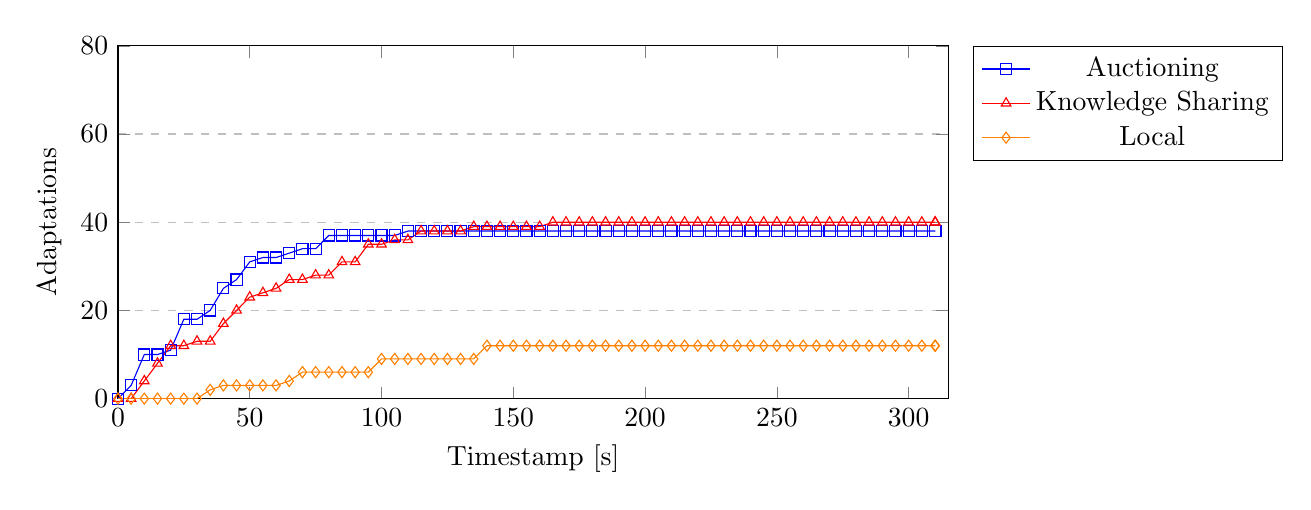
\begin{tikzpicture}
\begin{axis}[
    xlabel={Timestamp [s]},
    ylabel={Adaptations},
    xmin=0, xmax=315000,
    ymin=0, ymax=80,
    legend pos=outer north east,
    ymajorgrids=true,
    grid style=dashed,
    width=\textwidth,
    height=0.5\textwidth,
    scaled x ticks=base 10:-3,
    xtick scale label code/.code={}
]

	\addplot[color=blue,mark=square] coordinates {
        (0,0)(5000,3)(10000,10)(15000,10)(20000,11)(25000,18)(30000,18)(35000,20)(40000,25)(45000,27)(50000,31)(55000,32)(60000,32)(65000,33)(70000,34)(75000,34)(80000,37)(85000,37)(90000,37)(95000,37)(100000,37)(105000,37)(110000,38)(115000,38)(120000,38)(125000,38)(130000,38)(135000,38)(140000,38)(145000,38)(150000,38)(155000,38)(160000,38)(165000,38)(170000,38)(175000,38)(180000,38)(185000,38)(190000,38)(195000,38)(200000,38)(205000,38)(210000,38)(215000,38)(220000,38)(225000,38)(230000,38)(235000,38)(240000,38)(245000,38)(250000,38)(255000,38)(260000,38)(265000,38)(270000,38)(275000,38)(280000,38)(285000,38)(290000,38)(295000,38)(300000,38)(305000,38)(310000,38)(310169,38)
    };
    \addlegendentry{Auctioning}
	\addplot[color=red,mark=triangle] coordinates {
        (0,0)(5000,0)(10000,4)(15000,8)(20000,12)(25000,12)(30000,13)(35000,13)(40000,17)(45000,20)(50000,23)(55000,24)(60000,25)(65000,27)(70000,27)(75000,28)(80000,28)(85000,31)(90000,31)(95000,35)(100000,35)(105000,36)(110000,36)(115000,38)(120000,38)(125000,38)(130000,38)(135000,39)(140000,39)(145000,39)(150000,39)(155000,39)(160000,39)(165000,40)(170000,40)(175000,40)(180000,40)(185000,40)(190000,40)(195000,40)(200000,40)(205000,40)(210000,40)(215000,40)(220000,40)(225000,40)(230000,40)(235000,40)(240000,40)(245000,40)(250000,40)(255000,40)(260000,40)(265000,40)(270000,40)(275000,40)(280000,40)(285000,40)(290000,40)(295000,40)(300000,40)(305000,40)(310000,40)(310132,40)
    };
    \addlegendentry{Knowledge Sharing}
	\addplot[color=orange,mark=diamond] coordinates {
        (0,0)(5000,0)(10000,0)(15000,0)(20000,0)(25000,0)(30000,0)(35000,2)(40000,3)(45000,3)(50000,3)(55000,3)(60000,3)(65000,4)(70000,6)(75000,6)(80000,6)(85000,6)(90000,6)(95000,6)(100000,9)(105000,9)(110000,9)(115000,9)(120000,9)(125000,9)(130000,9)(135000,9)(140000,12)(145000,12)(150000,12)(155000,12)(160000,12)(165000,12)(170000,12)(175000,12)(180000,12)(185000,12)(190000,12)(195000,12)(200000,12)(205000,12)(210000,12)(215000,12)(220000,12)(225000,12)(230000,12)(235000,12)(240000,12)(245000,12)(250000,12)(255000,12)(260000,12)(265000,12)(270000,12)(275000,12)(280000,12)(285000,12)(290000,12)(295000,12)(300000,12)(305000,12)(310000,12)(310125,12)
    };
    \addlegendentry{Local}




\end{axis}
\end{tikzpicture}
    \caption{Graph showing the total amount of adaptations applied by agents in the scenario where no changes are made overtime.}
    \label{fig:proposals-no-change}
\end{figure}

From Figure \ref{fig:proposals-no-change} we can see that the knowledge-sharing agent applies the most adaptations, followed by the auctioning agent. The local-agent applies the least adaptations. The knowledge-sharing agent applies almost $3$ times  more adaptations than the local agent. The knowledge-sharing agent has a steep increase in the first $25$ seconds, after which it becomes more stable. The auctioning agent has a slower increase, but is applying adaptations at a steady rate. This is to be expected as any adaptation will be negotiated first, which takes time.

\begin{figure}[H]
    \centering
        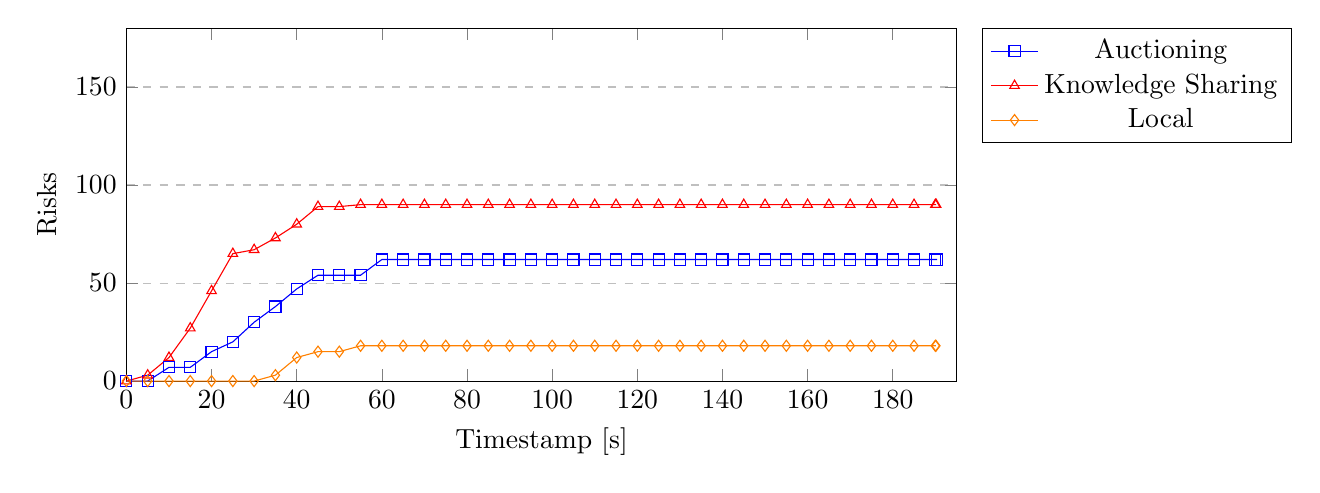
\begin{tikzpicture}
\begin{axis}[
    xlabel={Timestamp [s]},
    ylabel={Risks},
    xmin=0, xmax=195000,
    ymin=0, ymax=180,
    legend pos=outer north east,
    ymajorgrids=true,
    grid style=dashed,
    width=\textwidth,
    height=0.5\textwidth,
    scaled x ticks=base 10:-3,
    xtick scale label code/.code={}
]

	\addplot[color=blue,mark=square] coordinates {
        (0,0)(5000,0)(10000,7)(15000,7)(20000,15)(25000,20)(30000,30)(35000,38)(40000,47)(45000,54)(50000,54)(55000,54)(60000,62)(65000,62)(70000,62)(75000,62)(80000,62)(85000,62)(90000,62)(95000,62)(100000,62)(105000,62)(110000,62)(115000,62)(120000,62)(125000,62)(130000,62)(135000,62)(140000,62)(145000,62)(150000,62)(155000,62)(160000,62)(165000,62)(170000,62)(175000,62)(180000,62)(185000,62)(190000,62)(190434,62)
    };
    \addlegendentry{Auctioning}
	\addplot[color=red,mark=triangle] coordinates {
        (0,0)(5000,3)(10000,12)(15000,27)(20000,46)(25000,65)(30000,67)(35000,73)(40000,80)(45000,89)(50000,89)(55000,90)(60000,90)(65000,90)(70000,90)(75000,90)(80000,90)(85000,90)(90000,90)(95000,90)(100000,90)(105000,90)(110000,90)(115000,90)(120000,90)(125000,90)(130000,90)(135000,90)(140000,90)(145000,90)(150000,90)(155000,90)(160000,90)(165000,90)(170000,90)(175000,90)(180000,90)(185000,90)(190000,90)(190190,90)
    };
    \addlegendentry{Knowledge Sharing}
	\addplot[color=orange,mark=diamond] coordinates {
        (0,0)(5000,0)(10000,0)(15000,0)(20000,0)(25000,0)(30000,0)(35000,3)(40000,12)(45000,15)(50000,15)(55000,18)(60000,18)(65000,18)(70000,18)(75000,18)(80000,18)(85000,18)(90000,18)(95000,18)(100000,18)(105000,18)(110000,18)(115000,18)(120000,18)(125000,18)(130000,18)(135000,18)(140000,18)(145000,18)(150000,18)(155000,18)(160000,18)(165000,18)(170000,18)(175000,18)(180000,18)(185000,18)(190000,18)(190138,18)
    };
    \addlegendentry{Local}




\end{axis}
\end{tikzpicture}
    \caption{Graph showing the number of unique risks detected by agents in the scenario where no changes are made overtime.}
    \label{fig:risk-count-no-change}
\end{figure}

Figure \ref{fig:risk-count-no-change} shows that the knowledge-sharing agent detects the most risks, followed by the auctioning agent with roughly $70\%$ of the risks found. The local-agent detects the least amount of risks at only $10\%$ compared to the auctioning agent. It is to be expected that the local-agents can only detect a fraction of what the other agents detect, as the risks that can be deduced from only their local knowledge is limited.

\begin{figure}[H]
    \centering
        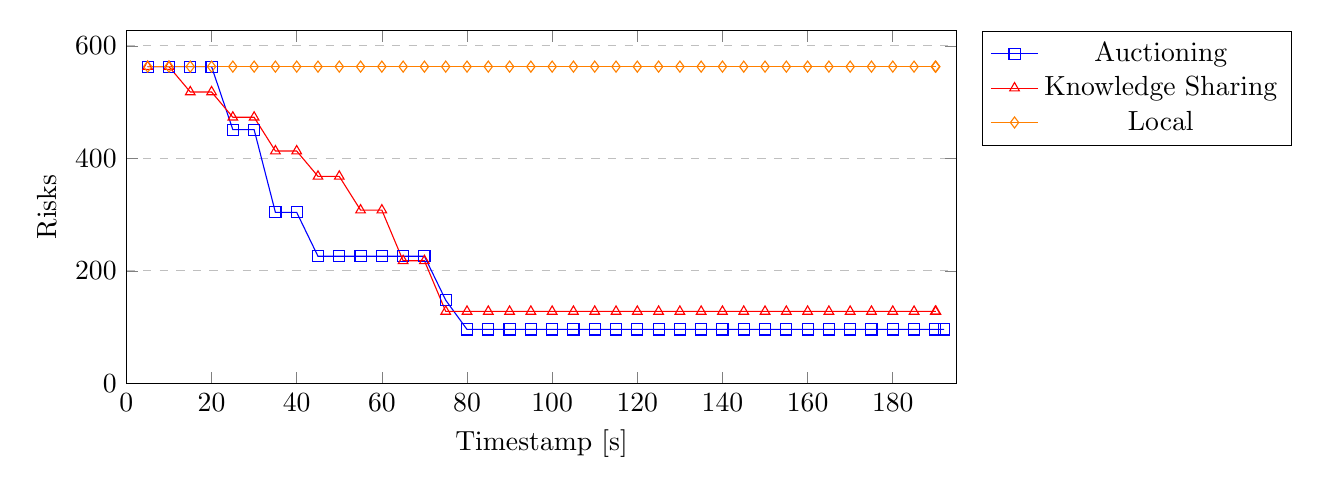
\begin{tikzpicture}
\begin{axis}[
    xlabel={Timestamp [s]},
    ylabel={Risks},
    xmin=0, xmax=195000,
    ymin=0, ymax=627,
    legend pos=outer north east,
    ymajorgrids=true,
    grid style=dashed,
    width=\textwidth,
    height=0.5\textwidth,
    scaled x ticks=base 10:-3,
    xtick scale label code/.code={}
]

	\addplot[color=blue,mark=square] coordinates {
        (5000,563)(10000,563)(15000,563)(20000,563)(25000,451)(30000,451)(35000,304)(40000,304)(45000,226)(50000,226)(55000,226)(60000,226)(65000,226)(70000,226)(75000,148)(80000,96)(85000,96)(90000,96)(95000,96)(100000,96)(105000,96)(110000,96)(115000,96)(120000,96)(125000,96)(130000,96)(135000,96)(140000,96)(145000,96)(150000,96)(155000,96)(160000,96)(165000,96)(170000,96)(175000,96)(180000,96)(185000,96)(190000,96)(192075,96)
    };
    \addlegendentry{Auctioning}
	\addplot[color=red,mark=triangle] coordinates {
        (5000,563)(10000,563)(15000,518)(20000,518)(25000,473)(30000,473)(35000,413)(40000,413)(45000,368)(50000,368)(55000,308)(60000,308)(65000,218)(70000,218)(75000,128)(80000,128)(85000,128)(90000,128)(95000,128)(100000,128)(105000,128)(110000,128)(115000,128)(120000,128)(125000,128)(130000,128)(135000,128)(140000,128)(145000,128)(150000,128)(155000,128)(160000,128)(165000,128)(170000,128)(175000,128)(180000,128)(185000,128)(190000,128)(190125,128)
    };
    \addlegendentry{Knowledge Sharing}
	\addplot[color=orange,mark=diamond] coordinates {
        (5000,563)(10000,563)(15000,563)(20000,563)(25000,563)(30000,563)(35000,563)(40000,563)(45000,563)(50000,563)(55000,563)(60000,563)(65000,563)(70000,563)(75000,563)(80000,563)(85000,563)(90000,563)(95000,563)(100000,563)(105000,563)(110000,563)(115000,563)(120000,563)(125000,563)(130000,563)(135000,563)(140000,563)(145000,563)(150000,563)(155000,563)(160000,563)(165000,563)(170000,563)(175000,563)(180000,563)(185000,563)(190000,563)(190111,563)
    };
    \addlegendentry{Local}




\end{axis}
\end{tikzpicture}
    \caption{Graph showing the number of remaining risks in the infrastructure in the scenario where no changes are made overtime.}
    \label{fig:risk-remaining-no-change}
\end{figure}

When comparing Figure \ref{fig:overall-damage-no-change} to Figure \ref{fig:risk-remaining-no-change}, we see that the graphs are following the same trend. This is to be expected, as the overall damage is calculated by summing the damage of all the remaining risks.

\begin{figure}[H]
    \centering
        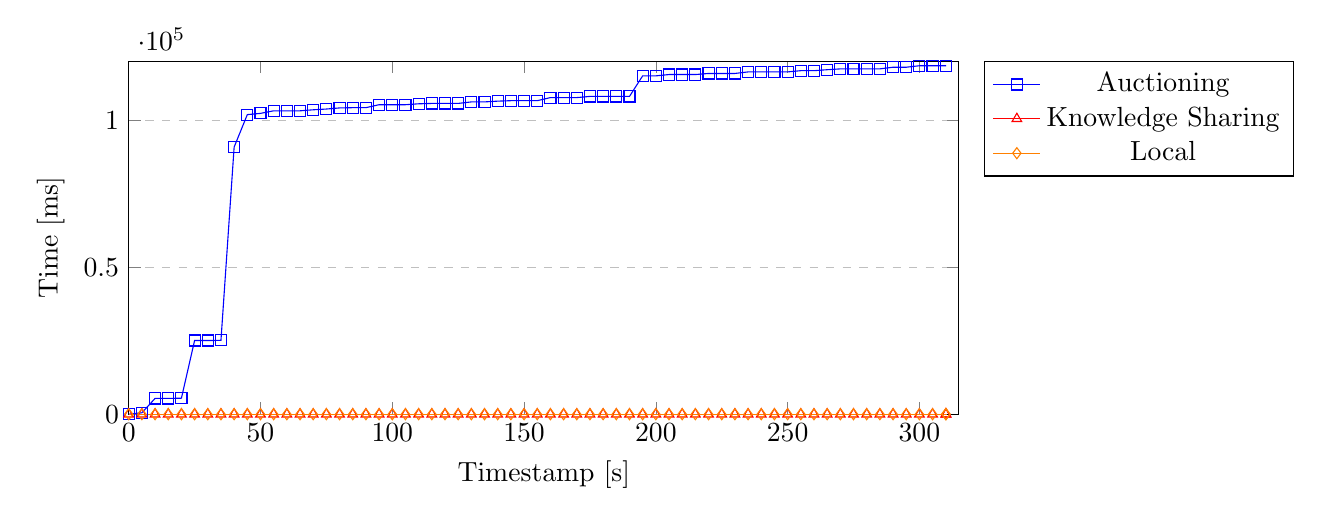
\begin{tikzpicture}
\begin{axis}[
    xlabel={Timestamp [s]},
    ylabel={Time [ms]},
    xmin=0, xmax=315000,
    ymin=0, ymax=120012,
    legend pos=outer north east,
    ymajorgrids=true,
    grid style=dashed,
    width=\textwidth,
    height=0.5\textwidth,
    scaled x ticks=base 10:-3,
    xtick scale label code/.code={}
]

	\addplot[color=blue,mark=square] coordinates {
        (0,0)(5000,475)(10000,5361)(15000,5361)(20000,5440)(25000,25066)(30000,25066)(35000,25093)(40000,90854)(45000,101889)(50000,102312)(55000,103185)(60000,103185)(65000,103185)(70000,103531)(75000,103788)(80000,104161)(85000,104251)(90000,104251)(95000,105263)(100000,105263)(105000,105263)(110000,105569)(115000,105695)(120000,105695)(125000,105695)(130000,106214)(135000,106214)(140000,106472)(145000,106629)(150000,106629)(155000,106629)(160000,107679)(165000,107679)(170000,107679)(175000,108080)(180000,108080)(185000,108080)(190000,108080)(195000,115072)(200000,115072)(205000,115518)(210000,115518)(215000,115518)(220000,115892)(225000,115892)(230000,115892)(235000,116415)(240000,116415)(245000,116415)(250000,116415)(255000,116836)(260000,116836)(265000,117162)(270000,117444)(275000,117444)(280000,117444)(285000,117444)(290000,118009)(295000,118009)(300000,118509)(305000,118509)(310000,118509)(310169,118509)
    };
    \addlegendentry{Auctioning}
	\addplot[color=red,mark=triangle] coordinates {
        (0,0)(5000,0)(10000,0)(15000,0)(20000,0)(25000,0)(30000,0)(35000,0)(40000,0)(45000,0)(50000,0)(55000,0)(60000,0)(65000,0)(70000,0)(75000,0)(80000,0)(85000,0)(90000,0)(95000,0)(100000,0)(105000,0)(110000,0)(115000,0)(120000,0)(125000,0)(130000,0)(135000,0)(140000,0)(145000,0)(150000,0)(155000,0)(160000,0)(165000,0)(170000,0)(175000,0)(180000,0)(185000,0)(190000,0)(195000,0)(200000,0)(205000,0)(210000,0)(215000,0)(220000,0)(225000,0)(230000,0)(235000,0)(240000,0)(245000,0)(250000,0)(255000,0)(260000,0)(265000,0)(270000,0)(275000,0)(280000,0)(285000,0)(290000,0)(295000,0)(300000,0)(305000,0)(310000,0)(310132,0)
    };
    \addlegendentry{Knowledge Sharing}
	\addplot[color=orange,mark=diamond] coordinates {
        (0,0)(5000,0)(10000,0)(15000,0)(20000,0)(25000,0)(30000,0)(35000,0)(40000,0)(45000,0)(50000,0)(55000,0)(60000,0)(65000,0)(70000,0)(75000,0)(80000,0)(85000,0)(90000,0)(95000,0)(100000,0)(105000,0)(110000,0)(115000,0)(120000,0)(125000,0)(130000,0)(135000,0)(140000,0)(145000,0)(150000,0)(155000,0)(160000,0)(165000,0)(170000,0)(175000,0)(180000,0)(185000,0)(190000,0)(195000,0)(200000,0)(205000,0)(210000,0)(215000,0)(220000,0)(225000,0)(230000,0)(235000,0)(240000,0)(245000,0)(250000,0)(255000,0)(260000,0)(265000,0)(270000,0)(275000,0)(280000,0)(285000,0)(290000,0)(295000,0)(300000,0)(305000,0)(310000,0)(310125,0)
    };
    \addlegendentry{Local}




\end{axis}
\end{tikzpicture}
    \caption{Graph showing the sum of time spent auctioning by agents in the scenario where no changes are made overtime.}
    \label{fig:auctioning-time-no-change}
\end{figure}

Figure \ref{fig:auctioning-time-no-change} shows that the auctioning agents is the only agent that spends time auctioning. This is to be expected, as the auctioning agents are the only agents that can auction.

\begin{figure}[H]
    \centering
        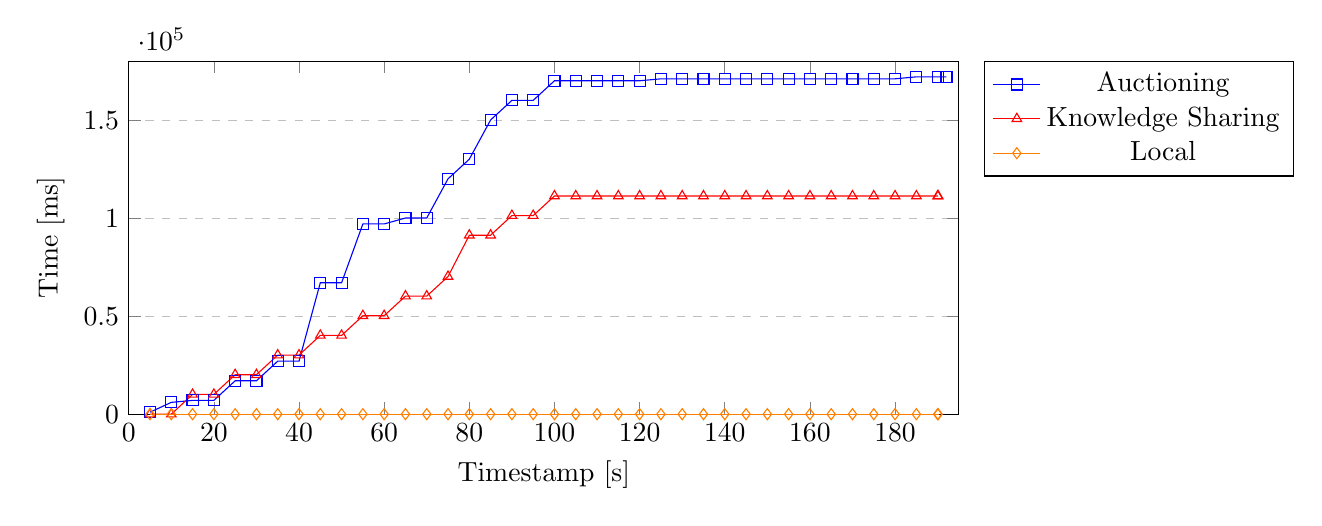
\begin{tikzpicture}
\begin{axis}[
    xlabel={Timestamp [s]},
    ylabel={Time [ms]},
    xmin=0, xmax=195000,
    ymin=0, ymax=180018,
    legend pos=outer north east,
    ymajorgrids=true,
    grid style=dashed,
    width=\textwidth,
    height=0.5\textwidth,
    scaled x ticks=base 10:-3,
    xtick scale label code/.code={}
]

	\addplot[color=blue,mark=square] coordinates {
        (5000,1004)(10000,6025)(15000,7027)(20000,7027)(25000,17033)(30000,17033)(35000,27038)(40000,27038)(45000,67055)(50000,67055)(55000,97062)(60000,97062)(65000,100075)(70000,100075)(75000,120080)(80000,130084)(85000,150091)(90000,160095)(95000,160095)(100000,170098)(105000,170098)(110000,170098)(115000,170098)(120000,170098)(125000,171100)(130000,171100)(135000,171100)(140000,171100)(145000,171100)(150000,171100)(155000,171100)(160000,171100)(165000,171100)(170000,171100)(175000,171100)(180000,171100)(185000,172103)(190000,172103)(192075,172103)
    };
    \addlegendentry{Auctioning}
	\addplot[color=red,mark=triangle] coordinates {
        (5000,0)(10000,0)(15000,10085)(20000,10085)(25000,20130)(30000,20130)(35000,30153)(40000,30153)(45000,40192)(50000,40192)(55000,50224)(60000,50224)(65000,60229)(70000,60229)(75000,70233)(80000,91314)(85000,91314)(90000,101317)(95000,101317)(100000,111324)(105000,111324)(110000,111324)(115000,111324)(120000,111324)(125000,111324)(130000,111324)(135000,111324)(140000,111324)(145000,111324)(150000,111324)(155000,111324)(160000,111324)(165000,111324)(170000,111324)(175000,111324)(180000,111324)(185000,111324)(190000,111324)(190125,111324)
    };
    \addlegendentry{Knowledge Sharing}
	\addplot[color=orange,mark=diamond] coordinates {
        (5000,0)(10000,0)(15000,0)(20000,0)(25000,0)(30000,0)(35000,0)(40000,0)(45000,0)(50000,0)(55000,0)(60000,0)(65000,0)(70000,0)(75000,0)(80000,0)(85000,0)(90000,0)(95000,0)(100000,0)(105000,0)(110000,0)(115000,0)(120000,0)(125000,0)(130000,0)(135000,0)(140000,0)(145000,0)(150000,0)(155000,0)(160000,0)(165000,0)(170000,0)(175000,0)(180000,0)(185000,0)(190000,0)(190111,0)
    };
    \addlegendentry{Local}




\end{axis}
\end{tikzpicture}
    \caption{Graph showing the sum of time spent adapting by agents in the scenario where no changes are made overtime.}
    \label{fig:adapting-time-no-change}
\end{figure}

Figure \ref{fig:adapting-time-no-change} shows that the knowledge-sharing agents spends the most amount of time adapting during this scenario. The auctioning agent is second, and the local agent spends the least amount of time adapting. This is inline with the amount of adaptations applied.
